\chapter[Considerações Finais]{CONSIDERAÇÕES FINAIS}

Quando ingressei na Engenharia de Software, meu interesse estava principalmente
na possibilidade de participar da construção e da manutenção de sistemas. Ao
longo das quatro etapas da AGES, compreendi que essa prática envolve muito
mais do que implementar funcionalidades. Um produto de software também depende
da compreensão do problema, da organização do trabalho, de decisões de
arquitetura, da integração entre diferentes partes da aplicação e, sobretudo,
da comunicação entre as pessoas envolvidas. Essa mudança de perspectiva foi a
principal contribuição da sequência de projetos para minha formação.

Na AGES I, entrei no projeto com pouca experiência nas tecnologias adotadas e
com dificuldade para encontrar uma forma concreta de contribuir. Minha timidez
e minha demora para pedir ajuda fizeram com que eu passasse tempo demais tentando
resolver sozinho uma tarefa de \textit{backend} que não consegui concluir. Quando
passei a concentrar meus estudos no \textit{frontend} e a trabalhar em dupla,
consegui participar da criação de componentes, da responsividade das telas e da
integração com as APIs. Essa primeira experiência me ensinou que reconhecer
um bloqueio e comunicá-lo cedo não é sinal de incapacidade. Também aprendi que
uma tarefa não está realmente pronta apenas porque funciona de forma isolada:
ela precisa ser integrada e testada com o restante da aplicação.

Na AGES II, procurei aplicar esse aprendizado desde o início. Tomei mais
iniciativa para conversar com os colegas, participei da modelagem conceitual e
lógica do banco de dados e, depois, da implementação de rotas, documentação e
revisões de código. Ao auxiliar colegas que enfrentavam dificuldades semelhantes
às que eu havia vivido, comecei a deixar a posição de quem apenas precisava de
orientação e passei também a servir como apoio. Ao mesmo tempo, percebi que ainda
me aproximava mais de alguns integrantes e poderia ter ajudado outras pessoas,
especialmente quando acumulávamos atrasos. Aprendi que não basta
estar disponível: em algumas situações, é necessário oferecer ajuda de forma
ativa e transformar os problemas apontados nas retrospectivas em mudanças no
modo de trabalhar.

A AGES III ampliou minha visão técnica do produto. Participei de decisões de
arquitetura, da preparação dos repositórios, do apoio aos integrantes menos
experientes e, principalmente, da infraestrutura na AWS e da automação de
\textit{deploy}. O trabalho exigiu estudar serviços de nuvem, Docker, GitLab
Runner e pipelines de CI/CD, além de realizar longas sessões de depuração.
Conseguimos automatizar o \textit{deploy} do \textit{backend}, mas a automação do
\textit{frontend} não foi concluída. Esse resultado me ensinou a distinguir
com mais cuidado o que foi planejado daquilo que realmente foi entregue. Também foi uma experiência difícil no aspecto interpessoal. Conflitos
no início do projeto me desmotivaram e fizeram com que eu evitasse algumas
discussões. Hoje reconheço que liderança técnica exige conhecimento, mas também
capacidade de sustentar uma decisão, ouvir objeções e lidar com discordâncias sem
abandonar o diálogo.

Na AGES IV, o foco deixou de estar em uma camada específica da aplicação e
passou a ser o funcionamento do time e do projeto como um todo. Trabalhei no
levantamento e na organização de requisitos, na preparação do backlog, no
acompanhamento das tarefas, na revisão e integração de contribuições, nos testes
em produção e na comunicação com o grupo. Considero que minha maior contribuição
foi manter as pessoas próximas: iniciei conversas, reuni o time, cobrei
atualizações e procurei preservar um ambiente leve, no qual pedir ajuda fosse
mais fácil. Por outro lado, minha maior falha foi não estruturar desde a Sprint 0
os épicos, as histórias e as tarefas com a granularidade necessária. A
organização adotada no ClickUp dificultou a visualização do trabalho durante
todo o semestre. As mobilizações próximas ao \textit{code freeze} mostraram que
trabalhar intensamente no final de uma sprint pode salvar uma entrega, mas não
substitui o acompanhamento contínuo. Na última sprint, concluir o desenvolvimento
com antecedência, testar o sistema integrado e preparar a demonstração com calma
confirmou essa diferença.

Ao observar as quatro experiências em conjunto, identifico uma evolução tanto
nas competências técnicas quanto nas interpessoais. Desenvolvi conhecimentos de
\textit{frontend}, integração com APIs, modelagem e persistência de dados,
desenvolvimento de \textit{backend}, revisão de código, arquitetura,
infraestrutura em nuvem, automação de entregas, requisitos, testes e gestão de
projetos. Entretanto, as habilidades que mais transformaram minha atuação foram
aprender a pedir ajuda, comunicar bloqueios, orientar colegas, dar e receber
\textit{feedback}, lidar com conflitos e tomar decisões. A comunicação aparece
em todos os capítulos deste memorial porque foi, ao mesmo tempo, uma das minhas
maiores dificuldades no início e minha contribuição mais forte ao final.

Essa evolução é sintetizada na Figura~\ref{fig:radar-evolucao}. O gráfico
representa uma autoavaliação acumulada das competências ao final de cada etapa,
em uma escala de 1 a 100. Os valores não correspondem a uma medição objetiva de
desempenho, mas à minha percepção sobre os conhecimentos e as habilidades que
desenvolvi durante os projetos.

\begin{figure}[H]
  \centering
  \small
  \caption{Autoavaliação da evolução das competências ao longo das etapas da AGES}
  \label{fig:radar-evolucao}
  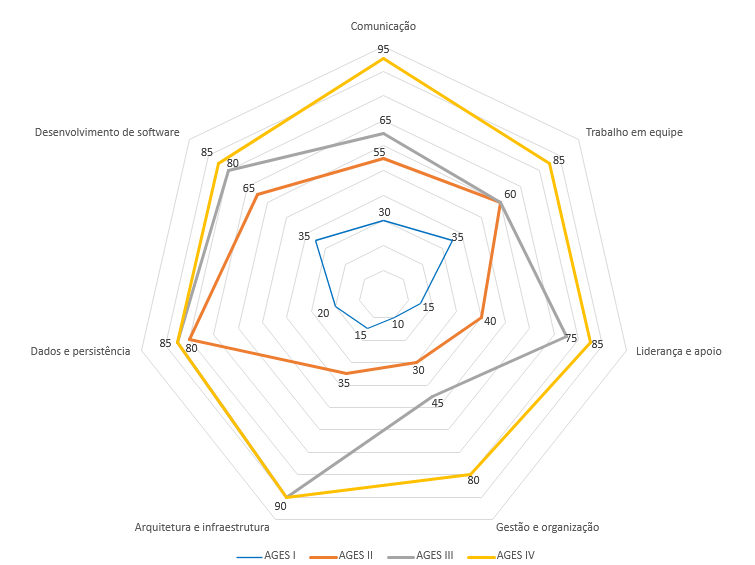
\includegraphics[width=1\linewidth]{conteudo/6 - consideracoes/figures/radar.png}
  Fonte: Elaborado pelo autor (2026)
\end{figure}

Minha visão da Engenharia de Software, portanto, deixou de estar centrada no
código. Continuo valorizando a solução técnica, mas hoje entendo que uma escolha
de tecnologia só faz sentido quando considera o problema, as restrições e as
pessoas que precisarão utilizá-la e mantê-la. Da mesma forma, aprendi que um bom
produto não significa necessariamente que o processo tenha sido bom. O Seniors
-- Empregabilidade terminou como um MVP completo dentro do escopo acordado e foi
muito bem recebido pelas \textit{stakeholders}, embora o semestre tenha exposto
problemas de organização, integração e colaboração. Em sentido inverso, até as
entregas incompletas ou os projetos mais desgastantes produziram aprendizados
que influenciaram diretamente minha atuação nas etapas seguintes.

Considero a proposta da AGES uma parte muito valiosa do curso. Trabalhar em
um problema apresentado por \textit{stakeholders} reais, com alunos em diferentes
níveis de experiência e com a responsabilidade de demonstrar um produto, criou
situações que dificilmente seriam reproduzidas apenas em exercícios isolados.
Também tive colegas prestativos e professores orientadores que tornaram essas
experiências mais ricas. A convivência entre AGES I, II, III e IV permite que o
aluno primeiro receba apoio e, progressivamente, assuma a responsabilidade de
apoiar outras pessoas. Para mim, essa foi uma das características mais
importantes da disciplina.

Ao mesmo tempo, acredito que essa progressão poderia ser mais bem sustentada por
orientações iniciais claras. Em diferentes semestres, faltaram referências
mínimas sobre tecnologias, artefatos obrigatórios, processos de infraestrutura
ou responsabilidades esperadas de cada etapa. Proatividade é necessária, mas é
difícil procurar uma informação cuja existência ou localização o aluno
desconhece. Sugiro que cada projeto comece com uma apresentação objetiva dos
papéis de AGES I a IV, dos artefatos exigidos, dos canais de apoio e do fluxo para
infraestrutura e arquitetura. Isso não retiraria a autonomia do time; daria uma
base comum para que a autonomia pudesse ser exercida. Também considero
importante acompanhar mais cedo se os alunos responsáveis pela liderança técnica
e pela gestão estão, de fato, orientando os iniciantes, revisando contribuições e
tornando os bloqueios visíveis.

Encerro essa trajetória com uma percepção mais realista sobre meu próprio modo
de trabalhar. Continuo valorizando a proximidade, o bom humor e a tentativa de
manter todos envolvidos, mas aprendi que liderar também exige firmeza. Tentar
agradar a todos pode adiar decisões necessárias, assim como evitar um conflito
pode permitir que um problema continue crescendo. O equilíbrio entre empatia e
decisão, entre dar autonomia e acompanhar o trabalho, é um aprendizado que ainda
pretendo desenvolver. Se na AGES I eu precisava vencer a insegurança para pedir
ajuda, ao final da AGES IV saio com a responsabilidade de criar condições para
que outras pessoas também consigam pedir, receber e oferecer essa ajuda.
